\chapter{Sistema de lectura de datos del robot}
\label{cap:lectura_datos}

Este capítulo entra en detalles técnicos de una de las tres funcionalidades principales de la estación diseñada: el sistema de muestreo y lectura de datos. Se comenzará haciendo una breve introducción al problema, comentando las variables de interés que se desean registrar y el funcionamiento deseado para el sistema. 

A continuación, se describirá el procedimiento que se ha empleado para utilizar ROS2 como cimiento de las señales registradas por el computador central de la estación. En la siguiente sección se presentará un caso de uso en el que se mostrará como resultado el registro de las variables seleccionadas anteriormente. Como punto final al capítulo, se comentarán las principales ventajas del sistema implementado, así como posibles mejoras por añadir en un futuro.

El código descrito en este capítulo se encuentra disponible en el repositorio GitHub del proyecto \cite{repo_github_TFM_MiguelLerinAlonso}. Los nodos de ROS2 que representan dichas tareas pertenecen al paquete \textit{data\_logger}\footnote{Disponible en el direccionamiento: \textit{./workspace/ros\_ur\_driver/src/data\_logger}}.

\section{Introducción al problema}
Actualmente las estaciones de fabricación deben registrar de forma continuada variables de importancia para el proceso que llevan a cabo. En el caso de las estaciones \acrshort{MEX}, estas variables suelen estar relacionadas con parámetros como pueden ser la posición del extrusor, la temperatura del material depositado o la altura de capa conseguida en cada nueva iteración.

El paradigma propuesto por los procesos \acrshort{NPAM} introduce ciertas modificaciones a las variables antes mencionadas. Dichas modificaciones cobran más relevancia especialmente si se trabaja con una plataforma de impresión móvil acoplada a un manipulador robótico, como puede ser el caso del presente proyecto.

De acuerdo con la arquitectura de control definida en el capítulo \ref{cap: diseno_arquitectura}, los datos provenientes de los sensores partícipes están involucrados con (1) la configuración cinemática adoptada por el robot en cada instante, (2) la información proveniente de la plataforma de impresión y (3) la lectura aportada por un sensor láser de distancia. Estas tres familias de datos de importancia deben procesarse por parte del computador central, que en última instancia será el responsable de su adecuada gestión.

Se busca la definición de una interfaz software que pueda gestionar aguas abajo del computador central toda esta información. La interfaz debe ser lo suficientemente flexible para permitir una lectura rápida de la información interna de la estación sin interferir en el proceso de fabricación que se esté llevando a cabo. En otras palabras, ha de integrarse con el movimiento del manipulador robótico y el control de temperatura de la cama de impresión.

\section{Metodología}
La construcción del sistema de lectura de datos presente en este proyecto atraviesa dos etapas diferenciadas. En la primera se seleccionan las variables de interés a las que debe poder acceder el sistema, al mismo tiempo se define el modelo de arquitectura de nodos ROS2 que se seguirá. La segunda etapa describe el proceso de creación de dicho sistema, haciendo especial en la escalada desde las unidades de código más atómicas hasta las de mayor nivel de abstracción.

\subsection{Selección de variables de interés}
Se procede al estudio de las capacidades de cada uno de los equipos hardware que participan en la estación robotizada, siendo aquellos que quedan dentro del alcance del proyecto el manipulador robótico UR, el sensor de distancia láser y la plataforma de impresión. Las variables de control de cada equipo, es decir, aquellas que pueden ofrecer información relevante sobre su estado son:

\begin{itemize}
    \item \textbf{Manipulador robótico:} Es el equipo responsable del movimiento de la plataforma de impresión según la trayectoria introducida y la velocidad comandada por el operario. Sus variables de interés serán aquellas que permitan definir de forma rápida su configuración cinemática en el espacio, como son la posición y velocidad de giro de cada articulación. Otras variables relacionadas con su comportamiento dinámico -como el caso de los esfuerzos articulares- también se consideran de interés de cara a futuros proyectos.
    \item \textbf{Sensor de distancia láser:} Este equipo permite validar la trayectoria efectuada por el manipulador robótico, midiendo la distancia existente entre el foco de energía láser y el punto de incidencia con la plataforma de impresión. Su variable de interés será dicha distancia.
    \item \textbf{Plataforma de impresión:} Su tarea principal es alcanzar y regular la temperatura comandada por el computador central. Es decir, la variable de interés es la temperatura registrada por el termopar en cada instante. Este dispositivo constituye uno de los componentes más modulares de la estación, por lo que se opta por dotarle de su propio sistema de comunicación con el computador central. La metodología seguida para dicha tarea se describe en el capítulo \ref{cap: control_temperatura}.
\end{itemize}

Se debe tener en cuenta que la frecuencia de actualización de cada variable puede depender directamente del equipo utilizado, por lo que será necesario emplear siempre una frecuencia de muestreo al menos dos veces superior a la de actualización del fenómeno registrado. En este caso, las principales limitaciones serán las aportadas por el \acrshort{PLC} integrado en el robot UR y la frecuencia de actualización impuesta en la unidad de control de la cama de impresión. Se considera que el procesador del computador central puede trabajar a una frecuencia más que suficiente para no ser una limitación.

Aprovechando la instalación existente en el laboratorio, se aprovecha la comunicación por MODBUS \acrshort{TCP/IP} para conectar directamente el computador central a la mesa de trabajo del manipulador robótico a utilizando un cable Ethernet. Este enfoque queda definido de cara a la interacción con otros equipos -como es el caso del sensor de distancia láser- que deben conectarse al \acrshort{PLC} del robot. El motivo principal por el que se selecciona esta solución es la necesidad de establecer un sistema de comunicaciones sencillo y confiable con un protocolo de comunicación industrial sobre el cuál ya habían trabajos previos para realizar sucesivas validaciones. 

Esto es, siguiendo la filosofía descrita por el capítulo \ref{cap: diseno_arquitectura} se busca que los componentes de la estación de fabricación puedan comunicarse entre sí sin necesidad de depender de elementos externos, como puede ser una conexión inalámbrica.

\subsection{Definición del sistema}
Con las variables de interés definidas se procede a evaluar el tipo de señal adecuado para cada una. Se tienen como factores de interés no solamente el equipo responsable de cada una, si no también su integración con diferentes protocolos de comunicación y equipos disponibles. En los siguiente párrafos se exponen el sistema de comunicaciones implementado para cada equipo, así como las razones detrás de la elección de una alternativa frente a otras.

\subsubsection*{Manipulador robótico}
\hypertarget{Manipulador robótico}{}
\bookmark[level=subsubsection,dest=Manipulador robótico]{Manipulador robótico}
Las configuraciones cinemáticas del manipulador robótico, así como la medida de sus esfuerzos articulares, son variables internas del equipo; motivo por el que su acceso no es inmediato y se debe disponer de una capa de software especializado en su registro y control. Con dicha limitación establecida, se opta por utilizar el entorno proporcionado por ROS2 Humble y en concreto, el controlador de UR para entornos de programación ROS2 \cite{UniversalRobots_ROS2_Driver}.

El controlador de UR basa su funcionamiento en una capa de software intermedia entre la versión de ROS2 empleada y el controlador Moveit, de modo que permite adaptar nodos de ambos sistemas a una versión específica para los equipos de la compañía. Dicha versión es capaz de gestionar automáticamente aspectos fundamentales de la definición del cobot como pueden ser sus ficheros de calibración, los controladores de movimiento o la lectura optimizada de variables internas. Esto resulta de gran utilidad no solamente para acceder de forma cómoda a valores articulares si no también a los diferentes registros de su \acrshort{PLC} integrado.

Puesto que la intención del sistema de registro de datos es elaborar un conjunto de solicitudes periódicas al robot UR que se vayan efectuando durante el tiempo de medida, se opta por emplear una arquitectura de ROS2 basada en el modelo publicador-suscriptor. En el modelo implementado en esta sección, el publicador será el robot, que deberá responder a la solicitud continuada del computador central proporcionando información en tiempo real. 

La información del manipulador, al estar directamente relacionada con los valores de posición, velocidad y esfuerzo articulares en cada instante de medida, debe responder a un nodo del entorno ROS2 especializado en dicho registro llamado \textit{joint\_states}. Siguiendo la terminología de ROS2, este nodo asume la tarea de publicador mientras que el paquete de lectura de datos -en concreto aquel nodo especializado en valores articulares- asumirá el papel de suscriptor. El nodo suscriptor se llama \textit{joint\_reader} y su funcionamiento queda descrito en el algoritmo \ref{alg:algoritmo_joint_reader}. 

\begin{algorithm}[H]
\caption{joint\_reader}\label{alg:algoritmo_joint_reader}
\begin{algorithmic}[1]
\Require Muestras totales que se desean realizar
\Ensure Vector de configuraciones articulares en tabla CSV

\State Arrancar el nodo como suscriptor de \textit{joint\_states}
\State Configurar la función de callback con el número de muestras deseadas

\While{Número de muestra $<$ Muestras totales}
    \State Leer configuraciones articulares de \textit{joint\_states}
    \State Almacenar valor leído en vector resultado
\EndWhile

\State Guardar vector resultado en tabla CSV

\end{algorithmic}
\end{algorithm}

El algoritmo \ref{alg:algoritmo_joint_reader} se presenta como una versión generalizada del procedimiento descrito, por lo que es fácilmente escalable a variables como posiciones, velocidades y esfuerzos articulares. El parámetro de entra principal es el número de muestras que se desean tomar, aunque también se definen otros valores como la ruta de guardado dentro del sistema de ficheros del computador central.

La Figura \ref{fig:nodo joint_reader rqt_graph} muestra en forma de grafo el conexionado del nodo \textit{joint\_reader} dentro del espacio de nodos que proporciona ROS2. Nótese cómo dicho nodo se suscribe únicamente el mensaje proveniente de \textit{joint\_states} y lo publica como una salida del sistema a través del mensaje genérico \textit{rosout}. De acuerdo con el firmware proporcionado por ROS2, en la parte superior de la imagen se muestra cómo interpreta a cada nodo y mensaje de forma automática. Siendo la publicación de \textit{joint\_states} un nodo de arquitectura publicador o \textit{publisher}, \textit{joint\_reader} el intermediario que hace las transformaciones necesarias entre el tipo de mensaje que se le proporciona y \textit{rosout} el escucha final ubicado aguas abajo al final de toda la información gestionada.

\begin{figure}[h!]
    \centering
    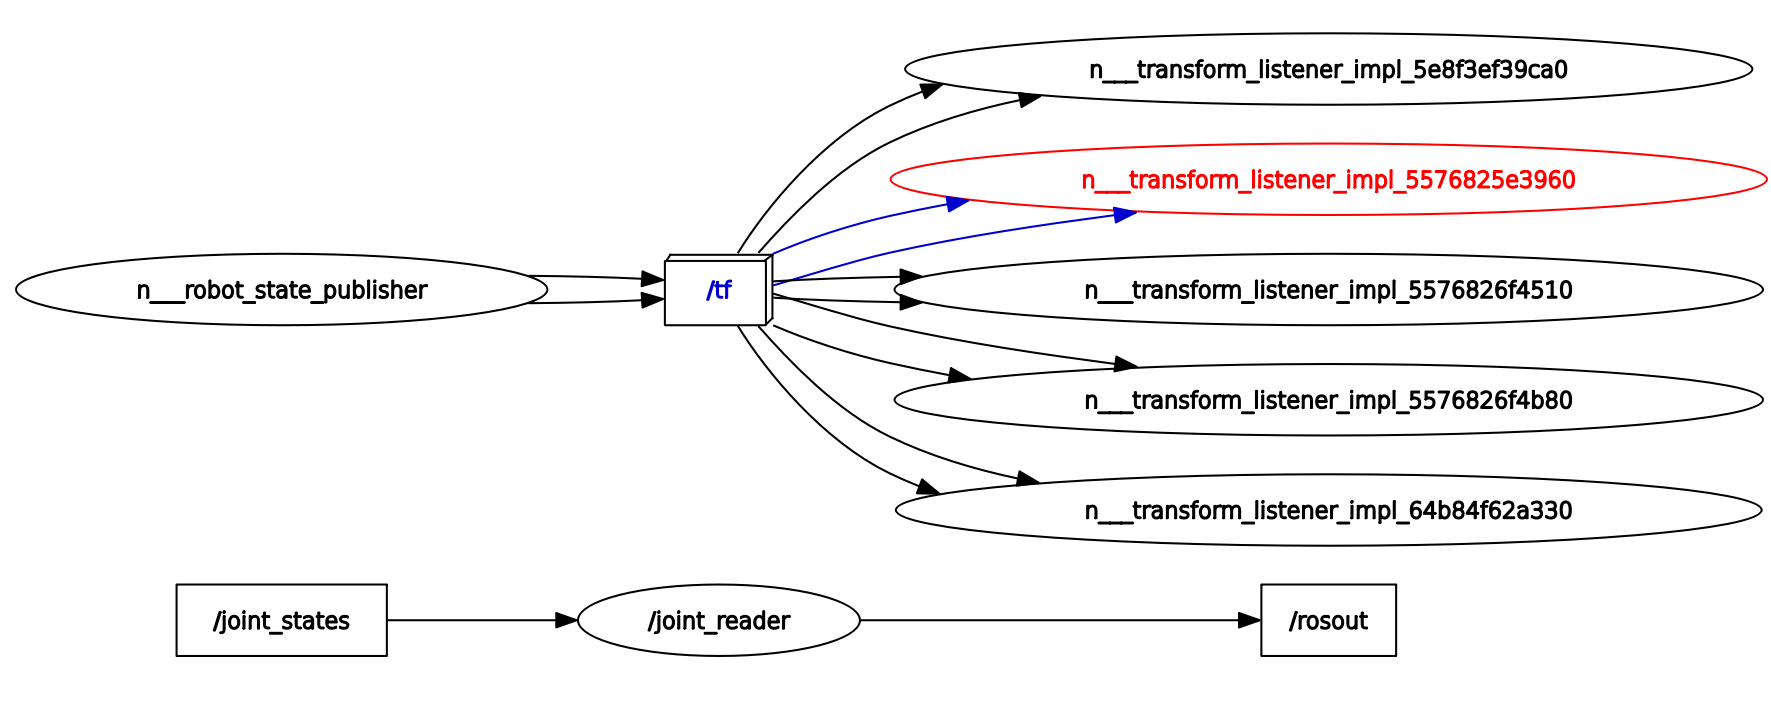
\includegraphics[scale=0.15]{figuras/nodo joint_reader rqt_graph.png}
    \caption{Grafo de estructuración del nodo \textit{joint\_reader}}
    \label{fig:nodo joint_reader rqt_graph}
\end{figure}


\subsubsection*{Sensor de distancia láser}
\hypertarget{Sensor de distancia láser}{}
\bookmark[level=subsubsection,dest=Sensor de distancia láser]{Sensor de distancia láser}

El sensor de distancia se caracteriza por enviar una señal analógica de corriente proporcional a la lectura. Al tratarse de un valor analógico que debe estar en constante comunicación con el manipulador robótico, se opta por conectarlo al \acrshort{PLC} a través de una de sus entradas digitales por mayor sencillez. La recta de calibración se muestra en la ecuación \ref{eq: calibracion sensor laser}.

\begin{equation}
\label{eq: calibracion sensor laser}
    d [m]=(0.035-0.025) \frac{I[A]-0.004}{0.02-0.004}+0.025 
\end{equation}

Es decir, se plantea un lector especializado en las entradas y salidas del \acrshort{PLC}. Este lector se sirve de la interfaz software proporcionada por el controlador de UR para ROS2, en concreto se accede al nodo \textit{/io\_and\_status\_controller/io\_states}. Este nodo proporciona una interfaz accesible tanto para entradas como para salidas, independientemente de si su naturaleza es digital o analógica. 

Por este motivo se plantea el algoritmo \ref{alg:algoritmo_analog_reader} como una referencia de funcionamiento tanto para señales digitales y analógicas. Los nodos de ROS2 responsable del muestreo de dichas señales se llaman respectivamente digital\_reader y analog\_reader. Ambos nodos reutilizan la estructura de publicador-suscriptor empleada en el lector de configuraciones articulares.

\begin{algorithm}[h!]
\caption{analog\_reader}\label{alg:algoritmo_analog_reader}
\begin{algorithmic}[1]
\Require Muestras totales que se desean realizar
\Ensure Vector de lecturas analógica

\State Arrancar el nodo como suscriptor de \textit{/io\_and\_status\_controller/io\_states}
\State Configurar la función de callback con el número de muestras deseadas

\While{Número de muestra $<$ Muestras totales}
    \State Leer valor de la señal muestreada
    \State Almacenar valor leído en vector resultado
\EndWhile

\State Guardar vector resultado en tabla CSV
\end{algorithmic}
\end{algorithm}

La Figura \ref{fig:nodo analog_reader rqt_graph} vuelve a utilizar el enfoque antes mencionado y muestra el grafo de conexionado entre los nodos responsables de lectura de puertos del \acrshort{PLC} y los nodos propios de ROS2 que proporcionan dicha información. 

\begin{figure}[h!]
    \centering
    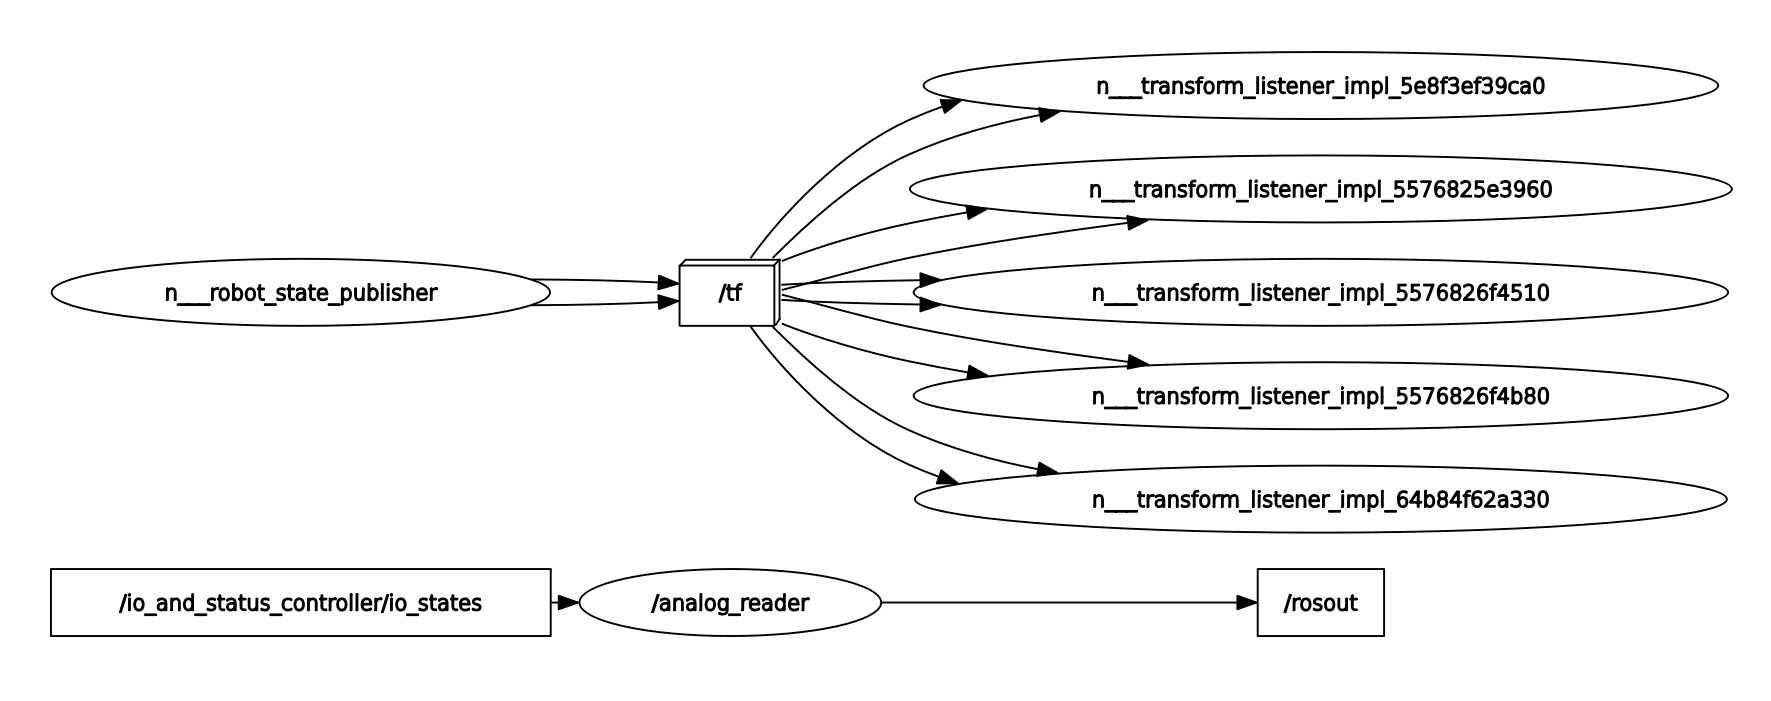
\includegraphics[scale=0.15]{figuras/nodo analog_reader rqt_graph.png}
    \caption{Grafo de estructuración del nodo \textit{analog\_reader}}
    \label{fig:nodo analog_reader rqt_graph}
\end{figure}

Cabe destacar que en este tipo de nodos se introducen nuevas configuraciones referentes a la frecuencia de muestreo, la definición del pin o si se trata de un valor de entrada o salida al \acrshort{PLC}. La definición de estos parámetros se explica con mayor detalle en el repositorio Git del proyecto\cite{repo_github_TFM_MiguelLerinAlonso}, en cuanto a la tarea de explicar el funcionamiento del sistema, no obstante dicha información se encuentra descrita y comentada en el repositorio del proyecto \cite{repo_github_TFM_MiguelLerinAlonso}.

\subsubsection*{Lectura del robot}
\hypertarget{Lectura del robot}{}
\bookmark[level=subsubsection,dest=Lectura del robot]{Lectura del robot}

Teniendo ya implementada una versión básica de lectores para cada tipo de datos provenientes de todos aquellos equipos de la estación relacionados directamente con el manipulador robótico, se procede a integrar dichos nodos de ROS2 en un esquema superior haciendo uso del soporte para \acrshort{POO}. Esto es, se define cada uno de los nodos antes descritos como una clase hija de una de mayor nivel de abstracción que pueda gestionar ambas al mismo tiempo. 

Esta nueva clase se conoce por el nombre de \textit{super\_logger} y se caracteriza por su capacidad de iniciar un registro en un proceso paralelo a la ejecución de trayectorias por parte del robot. La facilidad del nodo para realizar dicha tarea se debe a que integra dos nodos hijos que siguen el esquema de publicador-suscriptor, por lo que el propio nodo padre sigue dicho esquema. Dicho registro se puede definir a través de parámetros de interés como son el número de muestras deseadas, la frecuencia de muestreo, los pines del \acrshort{PLC} que se desean leer o el tipo de señal entre otros. 

El resultado de la lectura se guarda de forma predeterminada en una tabla CSV de forma automática\footnote{Disponible en el direccionamiento: \textit{./workspace/ros\_ur\_driver/src/data\_logger/results}}, aunque existe la posibilidad de indicar al sistema que continúe con el registro de datos por terminal una vez que haya guardado la tabla CSV. Los campos disponibles en dicha tabla son:

\begin{itemize}
    \item Número de muestra del registro
    \item Marca de tiempo en formato Unix
    \item Vector de posiciones articulares
    \item Vector de velocidades articulares
    \item Vector de esfuerzos articulares
    \item Estado de salida/entrada analógica
    \item Estado de salida/entrada digital
\end{itemize}

Cabe destacar que los vectores de configuraciones articulares constan de un total de 6 coordenadas, cada una correspondiente a una articulación del modelo definido en el entorno ROS2. Por comodidad en la lectura se opta por definir de forma predeterminada un único pin analógico y otro digital, ambos como salidas. No obstante el nodo está habilitado para admitir la introducción de parámetros personalizados a través de la terminal del computador central.

El algoritmo \ref{alg:algoritmo_super_logger} se utiliza para explicar el funcionamiento de dicho supernodo, se debe tomar en cuenta que utiliza como interfaz base la proporcionada por el controlador Moveit para ROS2 y los nodos de lectura del manipulador robótico antes descritos.

\begin{algorithm}[h!]
\caption{super\_logger}\label{alg:algoritmo_super_logger}
\begin{algorithmic}[1]
\Require Muestras totales que se desean realizar y frecuencia de muestreo
\Ensure Vector de lecturas analógica

\State Arrancar el nodo como suscriptor de \textit{joint\_states} y \textit{/io\_and\_status\_controller/io\_states}
\State Configurar la función de callback con el número de muestras deseadas

\While{Número de muestra $<$ Muestras totales}
    \State Leer valor de la configuración articular
    \State Formatear el valor de la configuración articular en forma de vector de seis componentes
    \State Almacenar valor leído en vector resultado para las configuraciones articulares

    \State Leer valor de señal analógica
    \State Almacenar valor leído en vector resultado de señal analógica
    \State Leer valor de señal digital
    \State Almacenar valor leído en vector resultado de señal digital

    \State Registrar marca de tiempo
    \State Registrar número de muestra
    
\EndWhile

\State Guardar vectores resultado en tabla CSV
\end{algorithmic}
\end{algorithm}

La Figura \ref{fig:nodo super logger} muestra el grafo de conexionado de este nodo con los mensajes de estados articulares y entradas/salidas del \acrshort{PLC} del manipulador robótico. Nótese cómo al invocar en su interior los nodos de lecturas articulares, analógicas y digitales se conserva el la tipología de los mensajes y la arquitectura publicador-suscriptor.

\begin{figure}[h!]
    \centering
    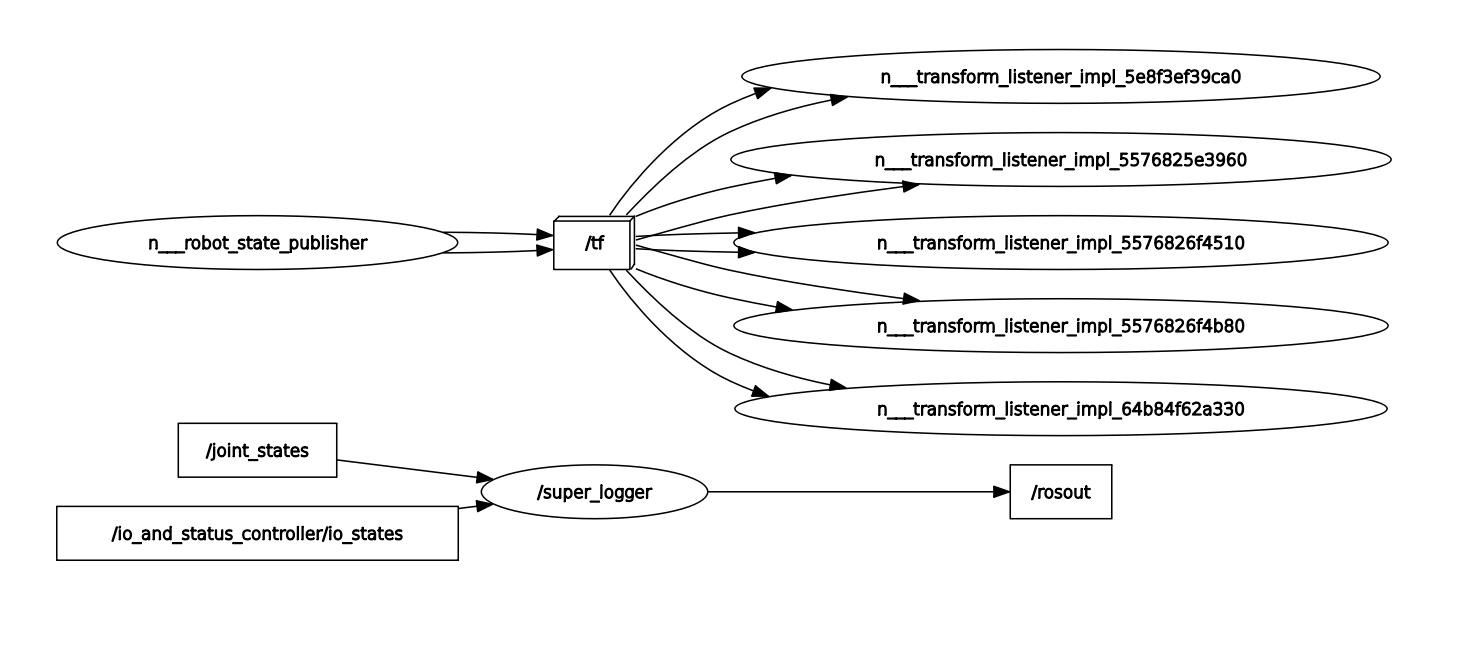
\includegraphics[scale=0.15]{figuras/nodo super_logger rqt_graph.png}
    \caption{Grafo de conexionado del nodo \textit{super\_logger}}
    \label{fig:nodo super logger}
\end{figure}

Este lector permite configurar el número de muestras necesarias para cubrir una trayectoria a partir de la frecuencia de muestreo y el tiempo de ejecución. El cálculo del número de muestras se muestra en la ecuación \ref{eq: tiempo_muestreo}. Donde $t$ es el tiempo en segundos que tarda en efectuarse la trayectoria, $n$ el número de muestras que se desean tomar y $f$ la frecuencia de muestreo en Hz.
Tanto la frecuencia como el número de muestras son parámetros accesibles al usuario, por su parte el tiempo de muestreo se deja a definición del usuario con ayuda de dicha ecuación.

\begin{equation}
\label{eq: tiempo_muestreo}
    N = f\cdot t
\end{equation}


\section{Resultados y conclusiones}
A continuación se evalúa el desempeño del sistema a través de la ejecución de una trayectoria de ejemplo. Posteriormente se indicarán las principales ventajas del sistema propuesto, así como algunas de sus posibles mejoras de cara a nuevas iteraciones del proyecto.

\subsection{Resultados}
Para evaluar el desempeño del sistema se establecen como marco común  dos movimientos del manipulador robótico a una frecuencia de muestreo de valor  limitado por el propio \acrshort{PLC} del manipulador, esto es 100 Hz. Dichos movimientos se realizan utilizando el entorno manipulación offline proporcionado por el controlador Moveit y la interfaz gráfica de Rviz.

La primera trayectoria cargará una trayectoria de compleja que se efectuará a altas velocidades. La segunda pondrá a prueba la medida proveniente del sensor láser desplazando a bajas velocidades la cama de impresión acoplada al manipulador.

\subsubsection*{Trayectoria helicoidal}
\hypertarget{Trayectoria helicoidal}{}
\bookmark[level=subsubsection,dest=Trayectoria helicoidal]{Trayectoria helicoidal}
A continuación se exponen el registro de datos de una trayectoria de mayor complejidad. Dicho movimiento tiene forma de hélice siguiendo las ecuaciones \ref{eq: Ecuaciones trayectoria sacacorchos} (representadas gráficamente en la Figura \ref{fig:trayectoria_sacacorchos_representacion}), y su cinemática ha sido definida siguiendo la metodología descrita en el capítulo \ref{cap: trayectorias}. Para clarificar el espacio de ejecución de la trayectoria elegida, la Figura \ref{fig: trayectoria sacacorchos entorno virtual} muestra posicionamiento con ayuda del entorno virtual definido con ROS2.

\begin{equation}
\label{eq: Ecuaciones trayectoria sacacorchos}
    \begin{align}
    x(t) &= R \cos(t) \\
    y(t) &= R \sin(t) \\
    z(t) &=  t
    \end{align}
\end{equation}

\begin{figure}[h!]
    \centering
     \begin{subfigure}[h]{0.45\linewidth} 
        \centering
        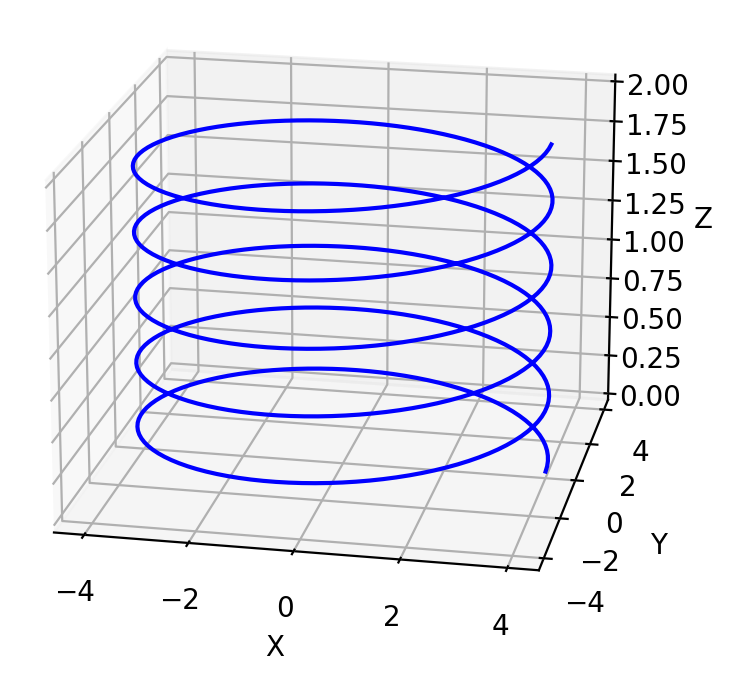
\includegraphics[scale=0.35]{figuras/ensayo_lectura_datos/trayectoria_sacacorchos.png}
        \caption{Representación gráfica}
        \label{fig:trayectoria_sacacorchos_representacion}
    \end{subfigure}
    \begin{subfigure}[h]{0.45\linewidth} 
        \centering
        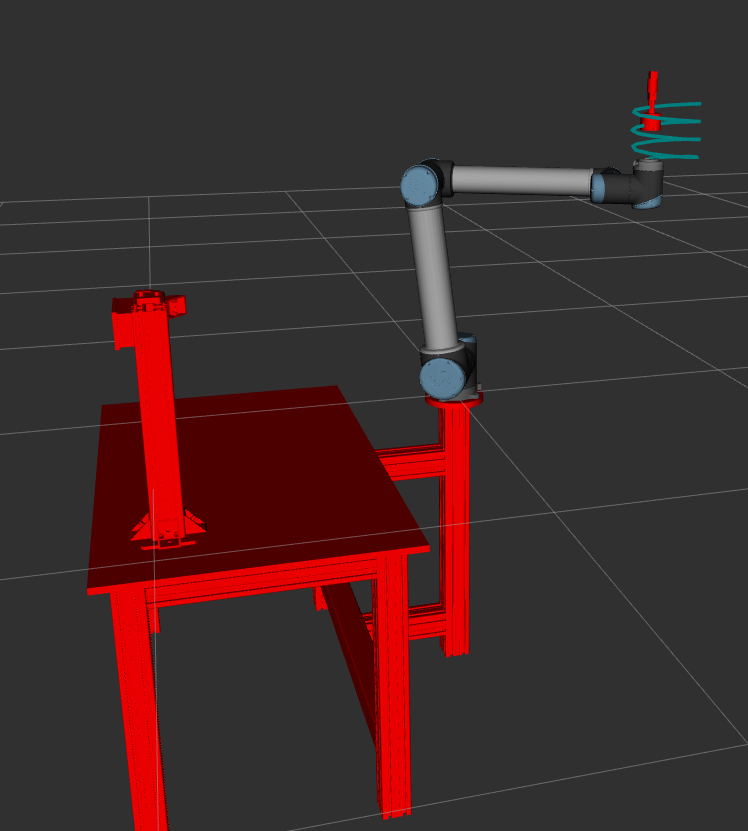
\includegraphics[scale=0.14]{figuras/trayectoria sacacorchos entorno virtual.png}
        \caption{Simulación en ROS2}
        \label{fig: trayectoria sacacorchos entorno virtual}
    \end{subfigure}
    \caption{Ensayo de lectura de configuraciones articulares}
\end{figure}

La cinemática calculada por la trayectoria expresa un movimiento cíclico de todas las articulaciones salvo por la \enquote{muñeca 1} del robot UR correspondiente a la articulación 2\footnote{Para aclaraciones sobre la numeración empleada en las articulaciones consultar la nota \ref{note: Aclaración número articulacionres ROS2}  del capítulo \ref{cap: trayectorias}}. Al ser responsable directo de la variación lineal de la cota Z de la trayectoria, se observa un cambio de posición lineal. Esta trayectoria se caracteriza por mantener la orientación del \acrshort{TCP} siempre constante, motivo por el que se espera que las articulaciones correspondientes a las  otras muñecas del UR (numeradas como 3 y 4) y la base (numerada como 5) varíen su posición cíclicamente con cada vuelta. Los resultados de dichas posiciones registradas pueden apreciarse en la Figura \ref{fig:trayectoria sacacorchos posiciones} y coinciden con el modelo esperado.

\begin{figure}[h!]
    \centering
    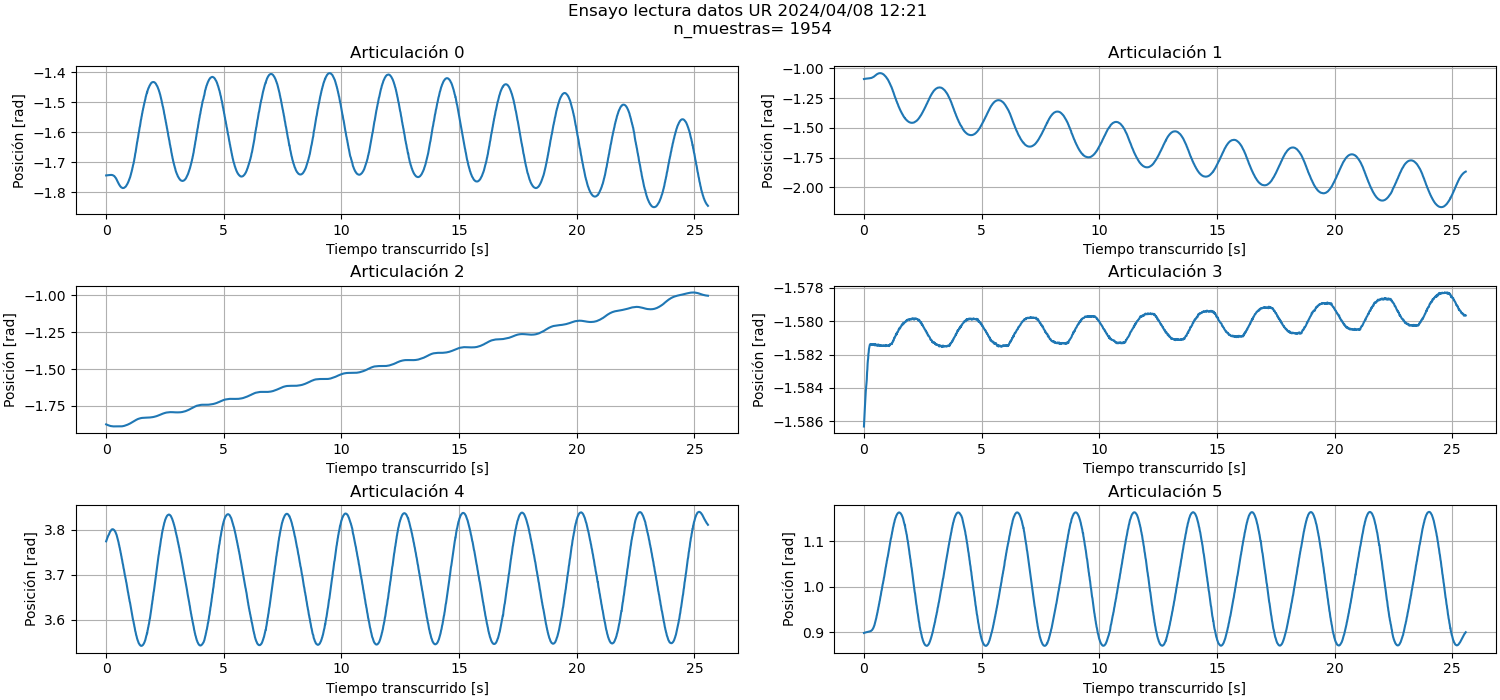
\includegraphics[scale=0.4]{figuras/ensayo_lectura_datos/posicion_sacacorchos.png}
    \caption{Posiciones registradas}
    \label{fig:trayectoria sacacorchos posiciones}
\end{figure}

El modelo también expresa la necesidad de un comportamiento constante y de pendiente prácticamente nula para la velocidad en la articulación 2. Del mismo también se esperan variaciones de tipo sinusoidales y muy suavizadas para las articulaciones de las muñecas del manipulador. 

La Figura \ref{fig:trayectoria sacacorchos velocidades} muestra la velocidad registrada por el sistema, se aprecia un buen desempeño en todas las articulaciones, habiendo obtenido curvas con la magnitud y comportamiento esperados. Cabe destacar los siguientes aspectos:
\begin{enumerate}
    \item Las velocidades asociadas a la \enquote{base} y al \enquote{hombro} del robot (numeradas como 0 y 1) muestran un comportamiento más suavizado que el resto. Este fenómeno se puede asociar a una velocidad mucho más reducida de sus actuadores, puesto que operan entre los $\pm$ 0.5 rad/s frente a los $\pm$ 10 rad/s del resto de articulaciones.
    \item Las altas velocidades alcanzadas por el resto de articulaciones (numeradas del 2 al 5)  favorecen la aparición de picos cuasi-instantáneos de velocidad. Se asocia la presencia de dichas discontinuidades a la aparición de aceleraciones articulares instantáneas que se desea compensar y la corrección efectuada por el propio controlador al tener en cuenta los límites establecidos por el descriptor del modelo robótico \acrshort{URDF}.
\end{enumerate}

\begin{figure}[h!]
    \centering
    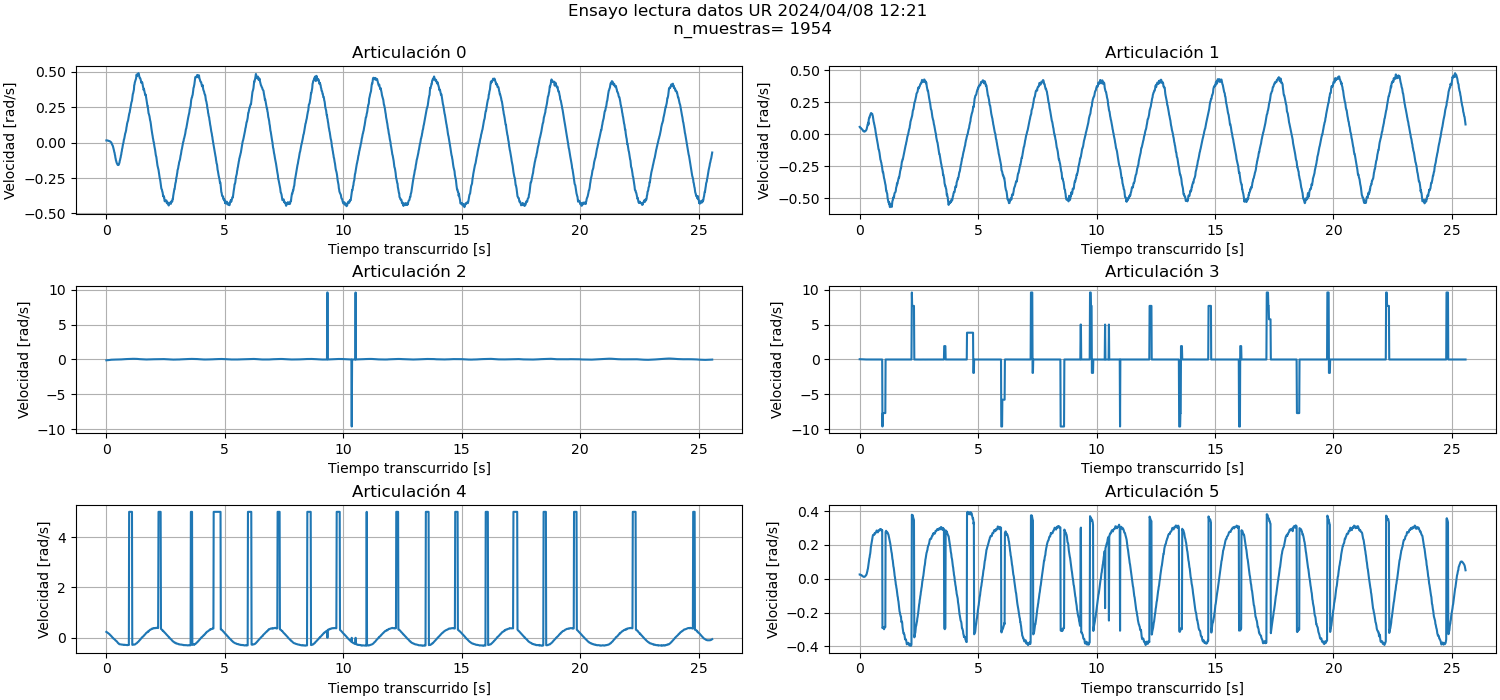
\includegraphics[scale=0.4]{figuras/ensayo_lectura_datos/velocidad_sacacorchos.png}
    \caption{Velocidades registradas}
    \label{fig:trayectoria sacacorchos velocidades}
\end{figure}

La Figura \ref{fig:trayectoria sacacorchos esfuerzos} muestra los esfuerzos registrados por sistema, en concreto se habla de torques articulares expresados en N-m. Se aprecia un comportamiento periódico y con un elevado rizado, este fenómeno se atribuye a la compensación de inercias que realiza el controlador constantemente.

\begin{figure}[h!]
    \centering
    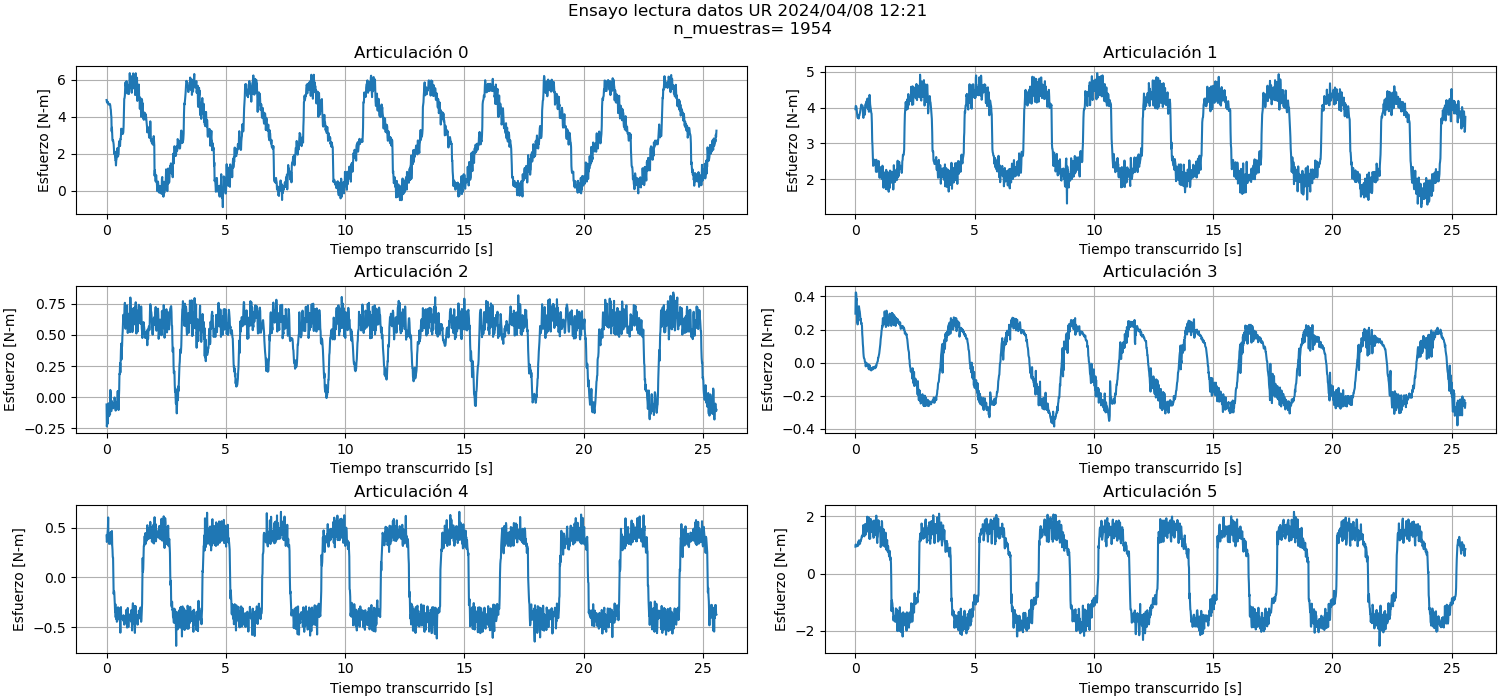
\includegraphics[scale=0.4]{figuras/ensayo_lectura_datos/esfuerzo_sacacorchos.png}
    \caption{Esfuerzos registradas}
    \label{fig:trayectoria sacacorchos esfuerzos}
\end{figure}

\subsubsection*{Distancia al sensor láser}
\hypertarget{Distancia al sensor láser}{}
\bookmark[level=subsubsection,dest=Distancia al sensor láser]{Distancia al sensor láser}
Finalmente, para validar el funcionamiento de entradas analógicas y digitales se procede a efectuar a desplazar la cama del sensor láser linealmente con ayuda del controlador Moveit y la interfaz gráfica de Rviz. En este caso se procede a programar dos poses que dejan el \acrshort{TCP} a una distancia concreta del sensor láser, de modo que el cobot se mueva alternativamente entre ellas. La operación se repite varias veces por intervalos variables de 10, 30, 60 y 90 segundos. La Figura \ref{fig:lectura con el sensor laser} muestra el desempeño de dicho ensayo, se observa que se mantienen unos valores similares a la lectura del sensor láser con un error aproximado del $\pm$3\%.

\begin{figure}[h!]
    \centering
    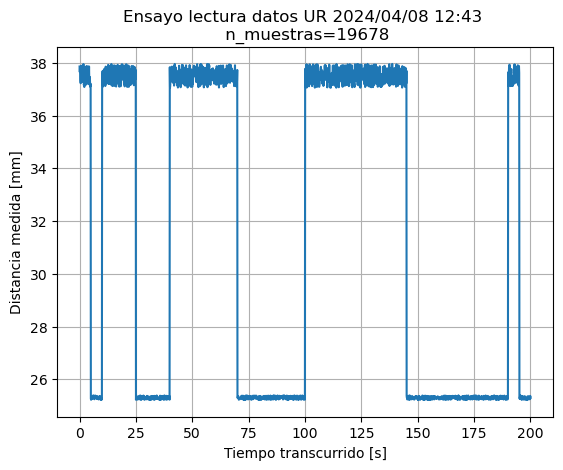
\includegraphics[scale=0.5]{figuras/ensayo_lectura_datos/lectura_datos_distancia_laser.png}
    \caption{Lectura con el sensor láser}
    \label{fig:lectura con el sensor laser}
\end{figure}

\subsection{Conclusiones}
El sistema implementado ha mostrado resultados similares a otros sistemas informáticos disponibles en el mercado \cite{ur_log_viewer_2024}. Asimismo, se observa que el uso de la arquitectura software fundamentada en ROS2 resulta lo suficientemente flexible para permitir la atomización del código en clases especializadas en la lectura de cada tipo de variable. Además, utilizando el enfoque de la \acrshort{POO}, se ha visto que se puede repetir este esquema en diferentes instancias, abriendo la puerta al desarrollo de un sistema de lectura de datos basado en ROS2 para diferentes equipos.

En consonancia con trabajos anteriores \cite{TFM_SanchoAmparo}\cite{TFM_Lu}, el sistema de lectura también se muestra capaz de detectar picos en los valores muestreados (como es el caso de las configuraciones cinemáticas) y puede combinar diferentes herramientas al mismo tiempo.

Algunas de las limitaciones observadas durante el desempeño del sistema han sido (1) la diferencia entre la frecuencia de muestreo asignada y la calculada por el ordenador y (2) la dependencia del entorno software empleado.

Se observa que en el momento de arranque existe un tiempo de aproximadamente 4 segundos en el que el nodo de muestreo de datos ha comenzado su función, pero todavía no se ha habilitado la transferencia de información del \acrshort{PLC} al computador central. Es decir, el retardo intrínseco de la señal es responsable de que las primeras muestras que se tomen durante dicho intervalo de tiempo -independientemente de la frecuencia de muestreo- aparezcan en el CSV como valores en blanco.

La Figura \ref{fig: limitacion_lectura_datos_frecuencia retardo} es un ejemplo de dicha problemática. En ella se muestran las lecturas de una trayectoria ensayada a una frecuencia de muestreo de 100 Hz. Se señala en color rojo la última muestra errónea, a partir de la cual comienza una lectura síncrona de la información proveniente del UR. El código empleado implementa un sistema de borrado de dicha información. Para el cálculo del tiempo transcurrido se utiliza la marca de tiempo como referencia. Dicha problemática ocurre a causa del retardo intrínseco de la señal, por lo que algunas soluciones adoptadas para minimizarlo pasan por:

\begin{itemize}
    \item \textbf{Arrancar el proceso desde una posición cercana al inicio de la trayectoria.} De este modo, se aprovecha el tiempo que transcurre hasta que el robot se ubica en el primer punto de la trayectoria objetivo para que las muestras correspondan a puntos sin interés.
    \item \textbf{Retrasar el arranque automático del muestreo de datos a través de código.} Si bien esta solución es fácilmente configurable, presenta como principal inconveniente la necesidad de definir un tiempo de espera característico para cada nueva trayectoria ensayada.
\end{itemize}

\begin{figure}[h!]
    \centering
    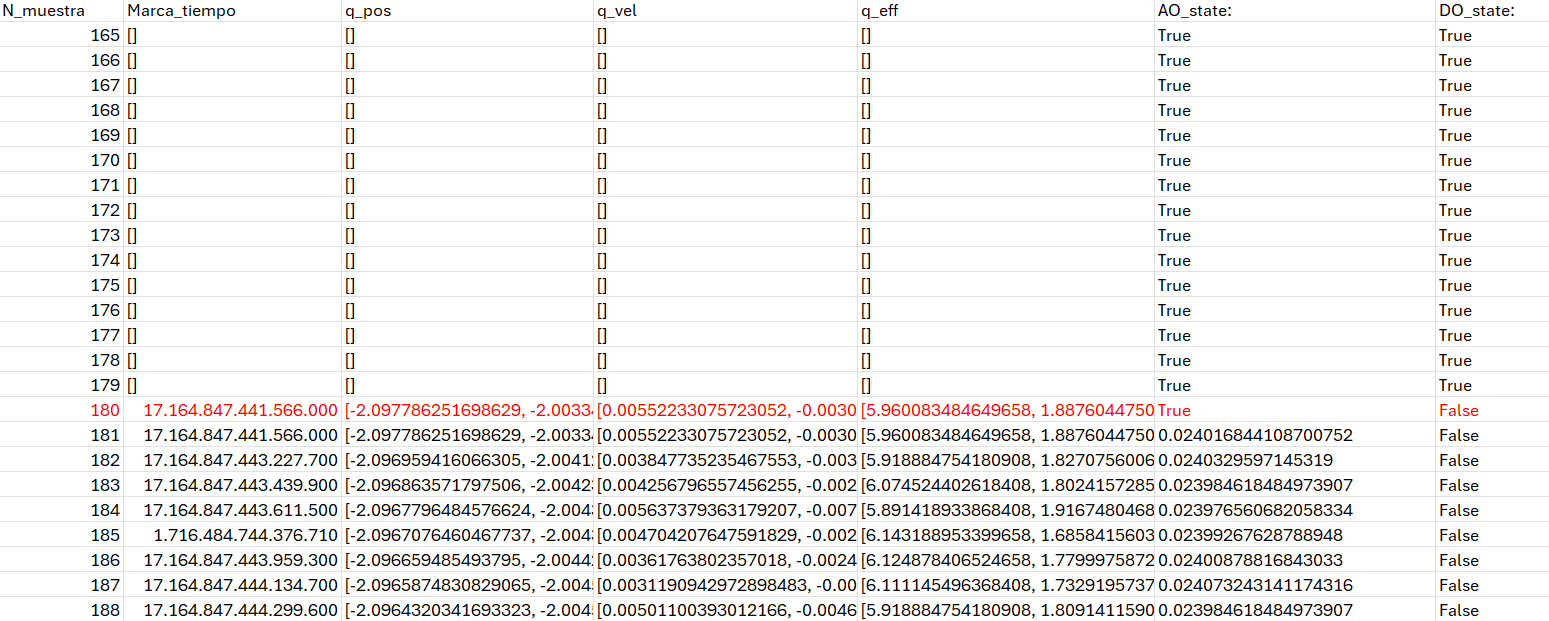
\includegraphics[scale=0.50]{figuras/ensayo_lectura_datos/limitacion_lectura_datos_frecuencia.png}
    \caption{Retardo en arranque de lectura de datos desde el \acrshort{PLC}}
    \label{fig: limitacion_lectura_datos_frecuencia retardo}
\end{figure}

Otra limitación asociada al sistema es la dependencia del entorno software ROS2 que se haya configurado en el computador central. Al utilizar los sistemas de lectura de estados del \acrshort{PLC} y de las articulaciones del propio manipulador, se debe definir cuidadosamente la calibración intrínseca del manipulador para minimizar el riesgo de medidas incorrectas o solape entre procesos. En robots comerciales -como el utilizado en este proyecto- no supone una gran limitación gracias a la capa intermedia de controladores desarrollada por la propia compañía. Esto es, puede suponer una ventaja al incorporar un sistema altamente validado, sencillo y con soporte que facilite la integración de nuevos equipos robóticos a la estación, aunque también puede suponer una limitación si el manipulador no dispone de dicha implementación.

Pese a las limitaciones observadas, los resultados obtenidos han demostrado ser satisfactorios y de fácil empleo. Por ello, se concluye que la lectura de datos se puede escalar y adaptar a tareas posteriores de mayor complejidad como el trazado de trayectorias en operaciones \acrshort{NPAM}.